\documentclass[twopage,11pt]{article}

% Any additional packages needed should be included after jmlr2e.
% Note that jmlr2e.sty includes epsfig, amssymb, natbib and graphicx,
% and defines many common macros, such as 'proof' and 'example'.
%
% It also sets the bibliographystyle to plainnat; for more information on
% natbib citation styles, see the natbib documentation, a copy of which
% is archived at http://www.jmlr.org/format/natbib.pdf

\usepackage{jmlr2e}
\usepackage{graphicx}% Definitions of handy macros can go here
\usepackage{hyperref}

\newcommand{\dataset}{{\cal D}}
\newcommand{\fracpartial}[2]{\frac{\partial #1}{\partial  #2}}

% Heading arguments are {volume}{year}{pages}{submitted}{published}{author-full-names}

\jmlrheading{1}{2008}{1-48}{4/00}{10/00}{RL-Glue Tanner and White}

% Short headings should be running head and authors last names

\ShortHeadings{RL-Glue}{Tanner and White}
\firstpageno{1}

\begin{document}

\title{RL-Glue Core \& Codecs 3.0 : Language Independent Software  for Reinforcement Learning Experiments}
% \title{The RL-Glue Software Project: An Open Source Framework for Reinforcement Learning Experiments}

%Title... I don't like framework because it sounds like you have to fit into it. One tentative title I had jotted down was:
%RL-Glue: Open source, language independent software for reinforcement learning experiments
%I like that one, but maybe it's not differentiated enough from the protocol.... but really, I disagree with Rich a bit here.  The software is called "RL-Glue", not "The RL-Glue software project". The debian package is rl-glue, the libraries are librlglue, the project is rl-glue.googlecode.com.
%I think it bogs down this paper to call it "The RL-Glue Software Project".
%That's how I'm feeling right now, sick, reading the title.

%Maybe we can tech it up.  I'm going back and changing it a different way.
%What about how it is now? With the 3.0?

\author{\name Brian Tanner \AND Adam White  \email \{btanner,awhite\}@cs.ualberta.ca \\
       \addr Department of Computing Science\\
       University of Alberta\\
       Edmonton, AB 98195-4322, Canada}

\editor{ Soeren Sonnenburg}

\maketitle

\begin{abstract}
%Note: will fix this later. still represents the paper well. but needs to be touched up
RL-Glue (Reinforcement Learning Glue) provides a standard interface that allows reinforcement learning agents, environments, and experiment programs to communicate with each other, even if they are written in different languages. The standardization provided by RL-Glue facilitates code-sharing and collaboration, reducing the need to re-engineer tasks and experimental apparatus from the literature in order to verify and compare-to the results of others.
%Brian stopped here.
RL-Glue is well suited for empirical research, course work and industrial scale projects. Our software features a minimalist interface and supports C, C++, Java, Python, Matlab and Lisp and runs on many computing platforms including Linux, Mac OS X, and Microsoft Windows. RL-Glue can be easily extended to support additional programming languages and other evaluation software using a TCP/IP interface. RL-Glue has been used to teach classes, to evaluate competitors in international reinforcement learning competitions and is currently used by several other open-source software and hardware projects.
\end{abstract}

\section{Introduction and Motivation}
In reinforcement learning an {\it agent} learns the effects of its {\it actions} through trial and error interaction with the {\it environment} [\cite{rlbook, rlsurvey,ndp}]. The agent selects actions based on its {\it observation} of the state of the environment and a scalar {\it reward} signal. The agent's objective is to select actions which maximize the sum of future rewards. The observations and rewards produced by the environment depend on the actions selected by the agent; the environment is not a static data-set, but rather a dynamic program that interacts with the agent.
%More differentiation from SL??
%Brian Feb 12 2009: I changed this a bit.  It's still not perfect.
%I moved away from the word "encoded", because technically every program is encoded as a file.  Pedantic, yes.
 


Different members of the reinforcement learning community use various incompatible software frameworks, making collaboration difficult and thus slowing the progress in our community. It is can be time consuming, difficult, and sometimes even impossible to exactly reproduce the work of others.  There is simply not enough space in the course of a conference publication to share a detailed specification of the environment, the agent, and the overall experimental apparatus.
Some reinforcement learning environments have become publicly available in different variations that are still each referred to, in the literature, as ``the standard", ``well-known" or ``classical"  versions [\cite{whiteThesis}]. %The RL-Glue Software Project is meant alleviate the evaluation difficulties facing reinforcement learning practitioners.
%Brian Feb 12 2009: This last sentence is important, or something like it is, to cap off the paragraph, but I really don't like that sentence.

%Maybe the motivation is strong enough that we dont need to talk about competitions and benchmarks...they are more difficult to defend anyway.
%There has also been significant interest, in recent years, in establishing annual agent competitions and benchmark problems, necessitating a standard evaluation system for reinforcement learning. 


%Brian: I think it's strong enough as is.




	 

\section{RL-Glue}

\begin{figure}[ht]
\begin{center}
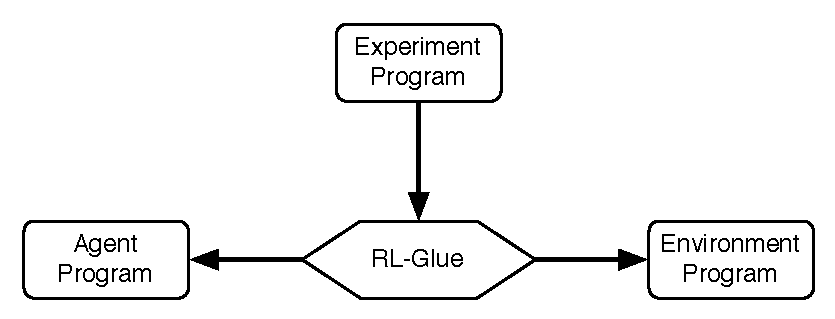
\includegraphics[width = 9 cm]{glue.pdf}
\vspace{-0.2cm}
\caption{\small The RL-Glue system architecture. Arrows indicate function call direction.}\label{fig:RLDIA}
\end{center}
\vspace{-0.4cm}
\end{figure}

%Brian: I agree with Shimon when he made this point about the AIM paper, we can't cite a paper that doesn't exist.  Perhaps you guys can release a tech report before this gets submitted.
The RL-Glue Software is an implementation of the RL-Glue Protocol [\cite{whitesutton}]. The RL-Glue Protocol is a standard for communication between agent and environment programs. The RL-Glue Protocol (illustrated in Figure \ref{fig:RLDIA}) separates the reinforcement learning framework into four main components: the agent program, environment program, experiment program and the RL-Glue interface. The agent program contains the learning algorithm and action selection mechanism. The environment program implements the dynamics of the task and generates the rewards. The experiment program controls the experiment's execution, including the sequence of agent-environment interactions and capturing statistical information about the agent's performance.  The RL-Glue interface mediates the communication between the agent and environment programs in response to commands from the experiment program. 

The RL-Glue Software can be run in either {\it native} or {\it network} mode. In native mode, the agent, environment and experiment program are compiled into a single C/C++ executable, and they communicate using function calls.  In networked mode, the agent, environment and experiment program communicate through RL-Glue over a TCP/IP socket connection. The network mode allows the agent, environment and experiment programs to be written in any programming language that supports socket I/O. The native mode can execute more steps per second, while the network mode is more flexible and portable. The agent and environment programs are completely agnostic of the execution mode.       

%This feels out of place, maybe it's better after the software intro... moving.
%Nope, still feels out of place, commenting out for now
%The RL-Glue Software is a language independent implemention of the RL-Glue Protocol  that allows agent, environment and experiment programs to be developed in different languages, and run on different computers over the internet. Please refer to the RL-Glue Software Project website for the latest code, documentation and subversion access:  {\url http://glue.rl-community.org/}

%This also felt out of place
%The current release of the RL-Glue Software includes support for Java, C/C++, Matlab, Python and Lisp. 

%UGH, I am not feelin this either.  Just feels not right here.  I will come back and try some things tomorrow
%The RL-Glue software also provides a means for sending the agent program a simple and concise message that describes the environment. The message allows the agent to, generally speaking, adapt itself to best learn about the environment.  This information can also be used to check that the agent and environment are compatible or provide the agent with prior information. A more complete description of RL-Glue's Task Specification Language can be found here: {\url http://glue.rl-community.org/Home/rl-glue/task-spec-language}.




\section{RL-Glue Software in Practice}
The RL-Glue Software Project has had a significant impact on the reinforcement learning community and has been used in several other projects. The reinforcement learning library\footnote{http://library.rl-community.org/} (RL-Libary) is a public repository of RL-Glue compatible agent, environment, experiment and utility programs.  The RL-Library is an open-source project that invites submissions from the reinforcement learning community. RL-Viz\footnote{http://code.google.com/p/rl-viz/} is an API layered on top of  RL-Glue, and can be used to dynamically load agent and environment programs, modify parameters at runtime and visualize interaction and performance.  The reinforcement learning competition\footnote{http://www.rl-competition.org/} is an annual event where teams from around the world compare their learning algorithms on a variety of challenging environments. The RL-Glue Software has been used as the evaluation system for all three competitions. Finally, the Critter Bot\footnote{\url{http://www.cs.ualberta.ca/~sokolsky/critterbot/}} is a mobile robot that is outfitted with a unusually rich set of subjective sensors. The Critter Bot is compatible with RL-Glue agents; agents developed for simulated environments can easily deployed to the robot.

The socket architecture of RL-Glue can also be used to connect agent programs to other software projects. Currently, socket bridges exist for connecting RL-Glue to a keepaway soccer server, a real-time strategy game engine and an Atari emulator. Our socket architecture helps lower the barriers for researchers wishing to work on larger scale environments by providing a simple and familiar interface. These environments will soon be accessible via RL-Library. 

The RL-Glue Software has been used for teaching reinforcement learning in several university courses and evaluating learning performance in scientific articles published in leading conferences. The RL-Glue website\footnote{\url{http://glue.rl-community.org/rl-glue-in-practice}} includes an updated list of all known projects that have benefited from RL-Glue.



\section{Other Reinforcement Learning Software Projects}
RL-Glue is not the only mature software project that aims to help standardize empirical reinforcement learning. CLsquare\footnote{\url{http://www.ni.uos.de/index.php?id=70}} provides much of the functionality of the RL-Glue Software, but only supports C++.
%CLSquare and the footnote are hard to work with.
PIQLE\footnote{\url{http://piqle.sourceforge.net/}} is a Java project that provides some of the functionality of the RL-Glue Software and supports multi-agent reinforcement learning. PIQLE, however, lacks important experiment control and support for real-valued action types. RL Toolbox\footnote{\url{http://www.igi.tugraz.at/ril-toolbox/}
} is a C++ object oriented system with many built-in learning algorithms, but does not support other programming languages or networked experiments.  The list of related projects goes on, and includes JRLF\footnote{\url{http://mykel.kochenderfer.com/jrlf/}}, LibPG\footnote{\url{http://code.google.com/p/libpgrl/}}, and probably others.

Some of these alternative packages are distributed with a number agents and environments which are of interest to RL-Glue users. RL-Glue has been designed with the goal of it being relatively easy to make existing programs RL-Glue compatible.  We are eager to offer assistance in bridging these frameworks to RL-Glue, with the hope of improving access to software for all members of our community.
%Ack this sounds pretty flowery.





 
 
 
\section{RL-Glue Open Source Project}
%NOTE: I am thinking about removing codecs from the paper ...
%Brian: I've noticed that its very low on codecs.  I think that's risky, but if you are pretty keen on it I'll see what I can do.

The RL-Glue Software is not just an evaluation tool or development environment: it is also a community project with many levels of possible participation. The easiest and most obvious way to participate is to submit agent, environment and experiment programs to the RL-Library. Developers can also extend the reach of RL-Glue  compatibility by writing socket-level interfaces for their favorite programming language.  The RL-Glue Software project also welcomes code submissions and improvements for all parts of the code base.   	

The RL-Glue Software Project has received significant contributions at many of the levels discussed above. The Lisp socket code was contributed by Gabor Balazs. Jose Antonio Martin H. developed a native windows implementation of the RL-Glue Software. The RL-Library has also received several environments submitted from previous competitions participants and paper authors. %Webpage detailing project contributions?
%Brian: That's a good idea. Very good.

%Brian: Obviously, this is  WAY out of place.
RL-Glue is available under the Apache License, Version 2.0.
	

\section{History of RL-Glue}
The RL-Glue Software project has gone through several iterations adding new features, supported languages and developers. The first release of the software, RL-Glue 1.0 in 2005, provided support for C/C++, Java and Python through a file-pipe interface. The primary contributors at the time were Adam White, Mark Lee and Richard Sutton. The next release of the software, RL-Glue 2.0 in 2007, introduced the socket communication architecture. RL-Glue 2.0 was created by White, Andrew Butcher, Lee, and Brian Tanner. The current release adds new languages (Matlab and Lisp), new example projects, platform-specific distributions, install programs, extensive documentation, and more.  The primary developer of RL-Glue 3.0 is Brian Tanner.
   



%\addcontentsline{toc}{chapter}{Bibliography}
     %add the above line to get "Bibliography" in the table of contents.
%
%\singlespacing % optional;  Bibliography is better in single spacing
               %            but you may choose different
               %            Don't use \singlespacing if your thesis
               %            is already in single spacing
%
                          % for long bibs.



\bibliography{jmlrTake2}



\end{document}  